\documentclass[12pt]{article}
 
\usepackage[margin=1in]{geometry} 
\usepackage{amsmath,amsthm,amssymb}

\usepackage[brazilian]{babel}
\usepackage[utf8]{inputenc}
\usepackage[T1]{fontenc}
\usepackage{graphicx}         %pacote para incluir figuras tipo eps
\usepackage{xcolor}
\usepackage{float} 
\usepackage{epstopdf}
\usepackage{longtable}
\usepackage{subcaption}

 
 %Matlab code in latex 
\usepackage[final]{listings}
\usepackage{color} %red, green, blue, yellow, cyan, magenta, black, white
\definecolor{mygreen}{RGB}{28,172,0}
\definecolor{mylilas}{RGB}{170,55,241}
\lstdefinestyle{myMatlab}
{
language=matlab,frame=single, basicstyle=\small\ttfamily,breaklines=true,%
morekeywords={matlab2tikz}, keywordstyle=\color{blue}, morekeywords=[2]{1}, keywordstyle=[2]{\color{black}}, commentstyle=\color{mygreen}, stringstyle=\color{mylilas}, identifierstyle=\color{black}, showstringspaces=false,%without this there will be a symbol in the places where there is a space
numbers=left, numberstyle={\scriptsize \color{black}},% size of the numbers
numbersep=9pt, % this defines how far the numbers are from the text
% emph=[1]{for,end,break},emphstyle=[1]\color{red}, %some words to emphasise
% emph=[2]{word1,word2}, emphstyle=[2]{style},
}
 
\newcommand{\N}{\mathbb{N}}
\newcommand{\Z}{\mathbb{Z}}
 
\newenvironment{theorem}[2][Theorem]{\begin{trivlist}
\item[\hskip \labelsep {\bfseries #1}\hskip \labelsep {\bfseries #2.}]}{\end{trivlist}}
\newenvironment{lemma}[2][Lemma]{\begin{trivlist}
\item[\hskip \labelsep {\bfseries #1}\hskip \labelsep {\bfseries #2.}]}{\end{trivlist}}
\newenvironment{exercise}[2][Exercício]{\begin{trivlist}
\item[\hskip \labelsep {\bfseries #1}\hskip \labelsep {\bfseries #2.}]}{\end{trivlist}}
\newenvironment{reflection}[2][Reflection]{\begin{trivlist}
\item[\hskip \labelsep {\bfseries #1}\hskip \labelsep {\bfseries #2.}]}{\end{trivlist}}
\newenvironment{proposition}[2][Proposition]{\begin{trivlist}
\item[\hskip \labelsep {\bfseries #1}\hskip \labelsep {\bfseries #2.}]}{\end{trivlist}}
\newenvironment{corollary}[2][Corollary]{\begin{trivlist}
\item[\hskip \labelsep {\bfseries #1}\hskip \labelsep {\bfseries #2.}]}{\end{trivlist}}
 
\begin{document}
 
% --------------------------------------------------------------
%                         Start here
% --------------------------------------------------------------
 
\title{Exercício 04}
\author{Renan Salles de Freitas\\
CPE 723 - Otimização Natural}
 
\maketitle
 
\begin{exercise}{1}
O objetivo deste exercício é escrever um programa de algoritmo genético simples.
O código de MatLab está abaixo:
\lstinputlisting[style=myMatlab]{matlab/ex1/ex1.m}

Como o código apresenta diversas funções e há várias maneiras de desenvolver o
código, é nencessário explicar comoo cada etapa do GA foi implementada. Como
parâmetros iniciais do algoritmoo, foi escolhida uma populaçãoo inicial de 10
indivíduos de 16 bits, com bit de maior valor significativo na esquerda. O
fenótipo é a conversão do gennótipo em números reais entre -2 e 2 e avalia-se
a função que se quer minimizar: $y = x^2 - 0.3\text{cos}(10\pi x)$. O código
MatLab para o fenótipo está abaixo:
\lstinputlisting[style=myMatlab]{matlab/ex1/mapbi2func.m}
\lstinputlisting[style=myMatlab]{matlab/ex1/bi2dec.m}
\lstinputlisting[style=myMatlab]{matlab/ex1/f.m}

Como é natural nos algoritmos genéticos, busca-se a minimização, portanto o
valor da função é negativado (linha 21 do código do exercício 1). Na próxima
etapa, guarda-se a melhor aptidão e o valor de $x$ real correspondente.

Na seleção de pais, optou-se por utilizar o algoritmo \textit{Amostragem
Estocástica Universal} (SUS). O ranking é feito com probabilidade, de acordo
com a aptidão. A implementaçãoo está abaixo:
\lstinputlisting[style=myMatlab]{matlab/ex1/sus_selection.m}
\lstinputlisting[style=myMatlab]{matlab/ex1/ranking.m}

A partir da geração de pais, a recombinação é feita se um um valor randômico for
menor que $p_c = 0.7$. Se isso acontecer, dois pais geram dois filhos por
recombinação do tipo 1 ponto (onde há troca da cauda dos bits). Aqui, optou-se
por representação binária Gray. Códigoo abaixo:
\lstinputlisting[style=myMatlab]{matlab/ex1/crossover.m} 

Caso o valor radômico não seja maior que $p_c$, o filho é uma cópia do pai.

Por fim, a mutação ocorre caso um valor randômico seja menor que $p_m = 0.001$.
Aqui também optou-se pela codificação Gray, já que alterações de um bit
representa números próximos em decimais. Códigoo abaixo:
\lstinputlisting[style=myMatlab]{matlab/ex1/mutation.m}

A função pode ser vista abaixo:
\begin{figure}[H]
    \centering
    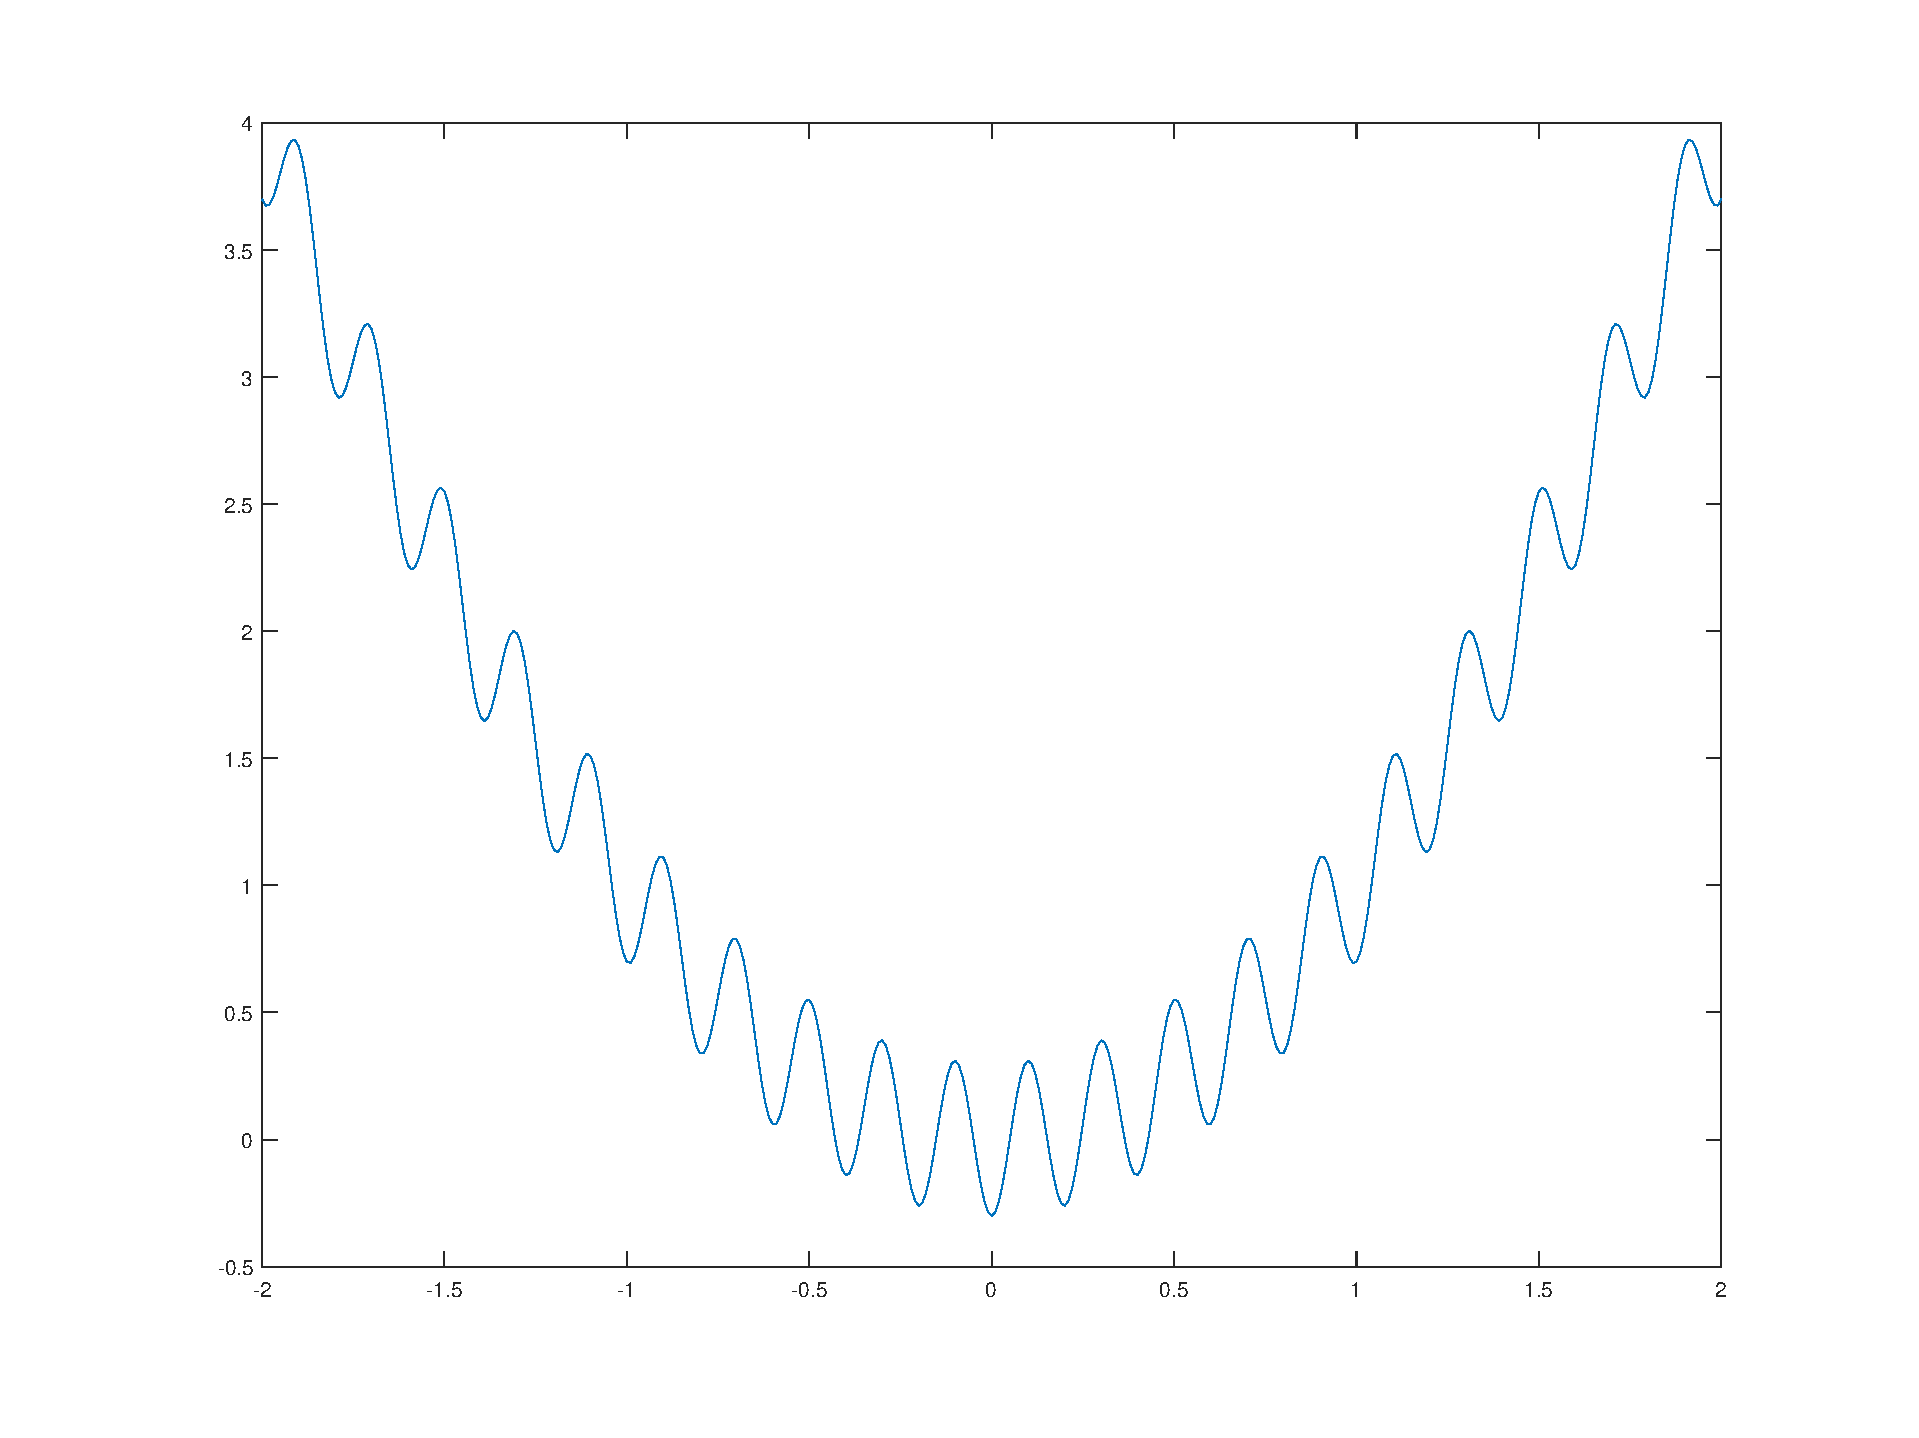
\includegraphics[width=0.5\textwidth]{figs/ex1.eps}
\end{figure}
\end{exercise}

Com uma população inicial de 10 indivíduos e realizando 100 iterações, obtemos
população final: $x = 0.0023$ e $f(x) = -0.2992$.

\begin{exercise}{2}
Exercício semelhante ao anterior, porém mudando parâmetros de população inicial
para 100, número de bits 25, função custo a ser maximizada (não minimizada) e,
por se tratar de uma função que usa a variável binária, não é necessário utilizar a codificação
Gray. Os códigos MatLab e gráficos são apresentados abaixo:

\lstinputlisting[style=myMatlab]{matlab/ex2/ex2.m}
\lstinputlisting[style=myMatlab]{matlab/ex2/f.m}
\lstinputlisting[style=myMatlab]{matlab/ex2/sus_selection.m}
\lstinputlisting[style=myMatlab]{matlab/ex2/ranking.m}
\lstinputlisting[style=myMatlab]{matlab/ex2/crossover.m} 
\lstinputlisting[style=myMatlab]{matlab/ex2/mutation.m}

\begin{figure}[H]
    \centering
    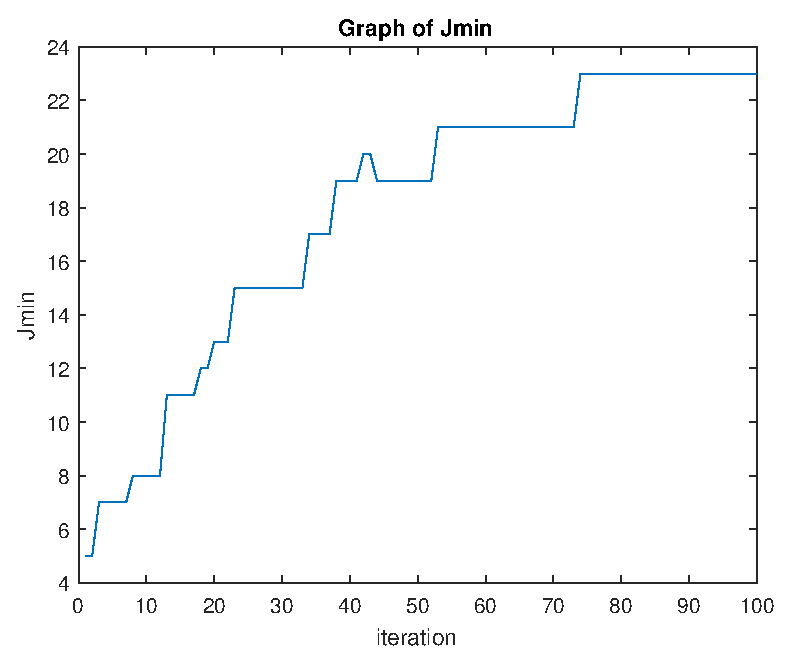
\includegraphics[width=0.5\textwidth]{figs/ex2_jmin.eps}
\end{figure}

\begin{figure}[H]
    \centering
    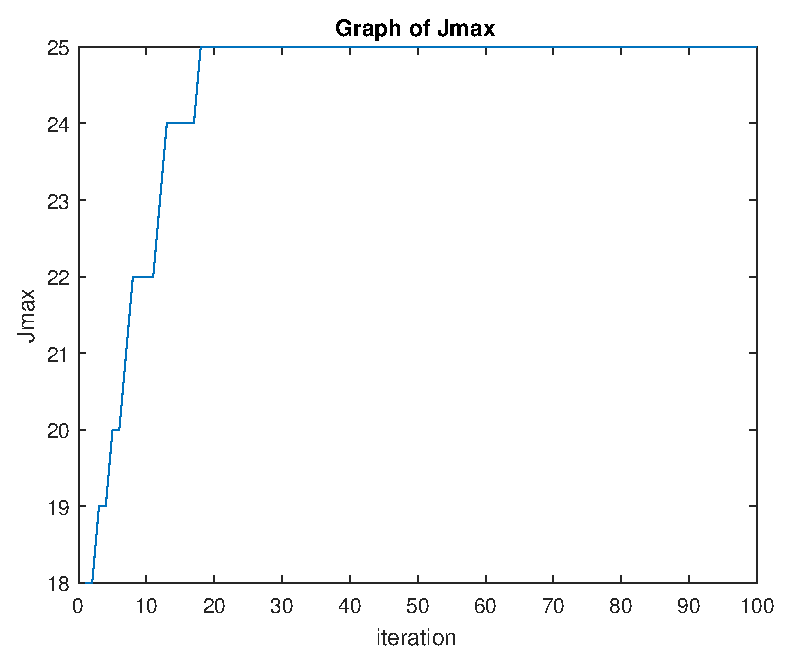
\includegraphics[width=0.5\textwidth]{figs/ex2_jmax.eps}
\end{figure}

\begin{figure}[H]
    \centering
    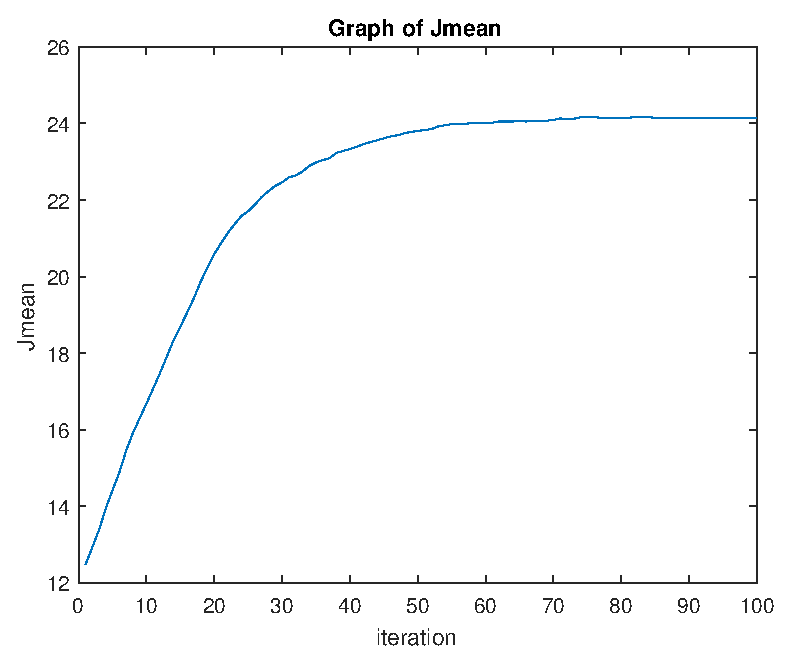
\includegraphics[width=0.5\textwidth]{figs/ex2_jmean.eps}
\end{figure}

A segunda parte do problema é rodar o algoritmo 10 vezes e verificar a média e
desvio padrão de iterações para o programa achar o ótimo gloobal.
Executou-se o código MatLab abaixo:
\lstinputlisting[style=myMatlab]{matlab/ex2/ex2b.m}

E foi encontrada média $19.2$ e desvio padrão $2.7406$.

\end{exercise}

\end{document}
              
